%SourceDoc ../YourName-Dissertation.tex
%\vspace*{-80mm}
\chapter{Introduction} \label{chapter1:introduction}

\section{\sloppy Motivation}
Titanium (Ti) and its alloys have been used in biomedical applications for many years because of their biocompatibility and corrosion resistance properties \cite{Long1998a}. In recent years, there has been an increasing interest in developing better materials for load-bearing implants, due to the increase in total knee and hip replacements. Krutz et al. predicted that the total number of hip and knee replacements would increase by 174\% and 673\%, respectively, from 2005 to 2030, leading to 572,000 hip and 3.48 million knee procedures in 2030 \cite{Kurtz2007}. Two of the driving factors for this situation are an increasing number of younger individuals requiring these replacements and the fact that the average life of total hip and knee replacements is only about 7-12 years before another replacement must be done \cite{Krishna2007a}. These factors all contribute significantly to the necessity for the development of better implant materials. The primary considerations for biomedical implants, such as load-bearing knee and hip implants, are biocompatibility, corrosion resistance, fatigue strength, and Young's modulus ($E$) \cite{Long1998a}. In previous years, the most common implants for these applications have been Ti-6Al-4V, stainless steels, and MoCoCr alloys \cite{Niinomi2003,Niinomi2012}. However, there have been issues with these materials, such as, cytotoxicity that has been observed with aluminum and vanadium \cite{Ito1995a}. Another important impediment concerning the common implant materials is stress shielding, which leads to implant failure. Stress shielding occurs when the $E$ of the implant is higher than that of bone. Due to the difference in $E$, load applications to the joint result in the implant material absorbing all of the stress and causing the bone surrounding the implant to atrophy, which leads to a loss in bone density, and can result in implant loosening and failure \cite{Long1998a}.  Table \ref{table:commonEM} summarizes the comparison of the $E$ of common implant materials (> 100 GPa) to bone (10-40 GPa) \cite{Long1998a}. This data indicates the extreme elasticity mismatch between the various materials. Computational thermodynamics and development of a knowledge base of Ti and its alloys will be useful tools in overcoming these challenges.

This work will focus on investigating the thermodynamics and elastic properties of the biocompatible Ti-Mo-Nb-Sn-Ta-Zr system. The thermodynamic and elastic properties will be calculated using first-principles based on Density Functional Theory (DFT). The parametrization of the properties will be completed using an integrated first-principles based on DFT calculations and CALPHAD modeling approach. The combination of these two methodologies has been shown to eliminate the need for trial-and-error metallurgy, thus saving time, money and other resources. New computational methodology to predict the metastable phase formation will be presented and verified by neutron scattering experiments. The culmination of this work will provide a fundamental understanding of the thermodynamics and elastic properties for the Ti-Mo-Nb-Sn-Ta-Zr system. 


\section{Overview}

The phase stability of Ti alloys has been seen to greatly influence the mechanical properties of the alloys and thus understanding the phase of a Ti alloy will greatly impact its effectiveness as a biomedical implant.


\subsubsection{Equilibrium Phases}

Titanium is stable in the $\alpha$ (hexagonal close packed, hcp) phase under the standard temperature and pressure. However, $\beta$ (body centered cubic, bcc) Ti alloys have received much attention because of their low \textit{E} and high specific strength and is thus targeted for the current application \cite{Mei2011,Brailovski2011b}. Mo, Nb and Ta are all biocompatible elements and considered strong $\beta$-stabilizers, while Zr is a bio-compatible weak $\beta$-stabilizer individually but strong stabilizer when in combination with other elements \cite{Long1998a}.  In conjunction with their bcc phase stability, Mo, Nb, Ta and Zr, in the presence of many non-toxic elements, studies have shown excellent corrosion resistance and no allergy problems \cite{Tane2008a}. Recently, tin (Sn) has also been studied for use in Ti-alloys, due to its biocompatibility and low cost \cite{Niinomi2012}. Due to these reason, the effects of alloying Ti with Mo, Nb, Sn, Ta and Zr on the thermodynamic properties were studied. The combined DFT and CALPHAD approach was used to evaluate previous models or build new models for the binary and ternary alloys in the Ti-Mo-Nb-Sn-Ta-Zr system to build a competed database describing the thermodynamic properties of the system.

\subsection{Elastic Properties}

The mechanical properties, in combination with studies of the various stable phases of Ti-alloys, have been experimentally determined for alloys such as Ti-13Nb-13Zr, Ti-35Nb-5Ta-7Zr-0.4O, Ti-29Nb-Ta-Zr and Ti-25Nb-Ta-Zr with Young's moduli between 71 and 57 GPa which starts to approach the $E$ of bone \cite{Long1998a,Tane2008a,Tane2010a}. While new metallic alloys are continually being designed, being able to predict the elastic properties before trying to make alloys for biomedical implants will reduce the need for trial and error and narrow down the scope of alloys being selected. With this goal in mind, this dissertation completes an extensive systematic study of the elastic properties of the pure elements, binary and ternary alloys in the bcc phase is completed using Density Functional Theory (DFT). Using the DFT data, CALPHAD modeling is then done to build a completed database that can predict the elastic properties as a function of composition.

\subsubsection{Metastable Phases}

While the thermodynamic database will predict the formation of the equilibrium phases and alloys in the bcc phase can then be targeted and their elastic properties predicted, Ti and its alloys form two metastable phases, $\alpha"$ and $\omega$. $\alpha"$ is an orthorhombic martensitic phase (space group Cmcm). The martensitic transformation is displacive and closely related to the system critical phenomenon \cite{Khachaturyan1985,Salje1990}. Thermodynamically the martensitic phase is a first-order transformation that is initiated due to some supercooling defined by $T_{0}-M_{S}$ where $T_{0}$ is the temperature where bcc goes to hcp and $M_{S}$ is the martensitic temperature where the martensitic transformation starts. An applied stress can also contribute to the driving force for a martensitic transformation. Kinetically the martensitic transformation propagates in an athermal manner which suggests that the velocity of the interface and the force causing its movement contain an instability. The $\omega$ phase is a metastable hexagonal phase (space group P6/mmm) of Ti that has lattice parameters closely matching that of bcc Ti. The $\omega$ phase has been seen to form athermally when Ti is alloyed with $\beta$ stabilizing elements such as Mo, Nb and Ta. The formation of $\omega$ and $\alpha"$ have been observed in Ti-Mo, Ti-Ta and Ti-Nb alloys. It is seen that different cooling of certain compositions of these binary alloys from a temperature in the single-phase bcc region to room temperature causes either the $\alpha"$ phase or the $\omega$ phase with the untransformed bcc phase. Quenching the samples leads to the formation of $\alpha"$ while slow cooling the sample leads to the $\omega$ phase. The formation of theses phases causes variations to the predicted elastic properties as seen in Figure \ref{Ch1-figure:titaelastic} where the closed symbols represent the calculated $E$ and the open symbols represent the experimentally determined $E$. The calculations and experiments match up well on the Ti-rich and Ta-rich sides of the graph but in the purple boxed region, the experiments show a much higher $E$ than predicted. This is due to the formation of $\alpha"$ and $\omega$. While the formation of the metastable phases greatly effects the properties of the Ti-alloys, the properties of unstable structures cannot be efficiently predicted by DFT-based first-principles calculations. In this dissertation, the phase stability and effect on the elastic properties of the $\alpha"$ and $\omega$ phases are studied for the Ti-Nb and Ti-Ta systems. First, the ground state energy and elastic properties of multiple structures in the $\alpha"$, $\omega$, bcc and hcp are calculated, across all compositions, for the Ti-Ta and Ti-Nb systems. The partition function approach is then adapted to predict the concentrations and phases fractions where the metastable phases are likely to form. The predicted phase fractions are then used to predict the elastic modulus and phonon density of states using a rule of mixtures. The predictions are confirmed with inelastic neutron scattering experiments. By looking at the diffraction patterns obtained at 300 $^\circ$K the phase fractions can be obtained and compared to the predicted phase fractions. The phonon density of states (DOS) obtained from neutron scattering experiments at 300 $^\circ$K can be compared with a mixed force constant first-principles phonon density of states. The plotting of the phonon density of states obtained through neutron scattering at different temperatures will be analyzed to help further understand the transformations taking place.


\pagebreak
\section*{This completed thesis will consist of the following main tasks:}

\begin{enumerate}
	\item Using first-principles calculations based on DFT and the CALPHAD method to investigate the thermodynamics of the Ti-Mo-Nb-Sn-Ta-Zr system. 
	\begin{enumerate}
		\item The previous binary models will be evaluated with the available experimental data as well as the first-principles calculated enthalpy of formation of the bcc phase
		\item The thermodynamic description of the Sn-Ta binary alloy will be modelled
		\item The thermodynamic descriptions of the Ti-containing ternary alloys will be modelled
	\end{enumerate}
	\item Using first-principles calculations the elastic properties of the Ti-Mo-Nb-Sn-Ta-Zr system in the bcc phase will be systematically studied. The results, as well as the CALPHAD method, will be used to build a database to predict the elastic properties as a function of composition. 
	\item The metastable phase formation in Ti alloys will be investigated through first-principles calculations, the CALPHAD method and experiments done on the Ti-Nb and Ti-Ta systems
	\begin{enumerate}
		\item The ground state energy and elastic properties of the Ti-Nb and Ti-Ta systems in the hcp, bcc, $\omega$ and $\alpha"$ will be predicted using first-principles calculations
		\item From first-principles the:
			\begin{enumerate}
			\item Adapted partition function approach will predict the phase fractions
			\item The phase fractions will be used in a rule of mixtures to plot the phonon density of states and elastic properties
		\end{enumerate}
		\item From neutron scattering:
		\begin{enumerate}
			\item The phase fractions will be determined and compared to the predictions
			\item The phonon density of states will be plotted at 300 $^\circ$K to compare to the mixed force constant predicted phonon density of states 
			\item The temperature dependent phonon density of states will be plotted to study the transformation 
		\end{enumerate}
	\end{enumerate} 
\end{enumerate}
				
\pagebreak
\begin{table}[H]
	\caption{Young's modulus of common implant materials compared with the Young's modulus of bone \cite{Long1998a}.}
	\centering
	\begin{tabular}{ c c }
		\hline
		Alloy & Young's Modulus (GPa) \\
		\hline
		Bone & 10-40\\
		cp-Ti* & 105\\
		Ti-6Al-4V & 110\\
		Stainless Steel & 200\\
		CoCrMo & 200-230\\
		\hline
		*cp-commercially pure titanium 
	\end{tabular}
\label{table:commonEM}
\end{table}
%%%
\clearpage

\newpage
%%%
\begin{figure}[H]
	\centering
	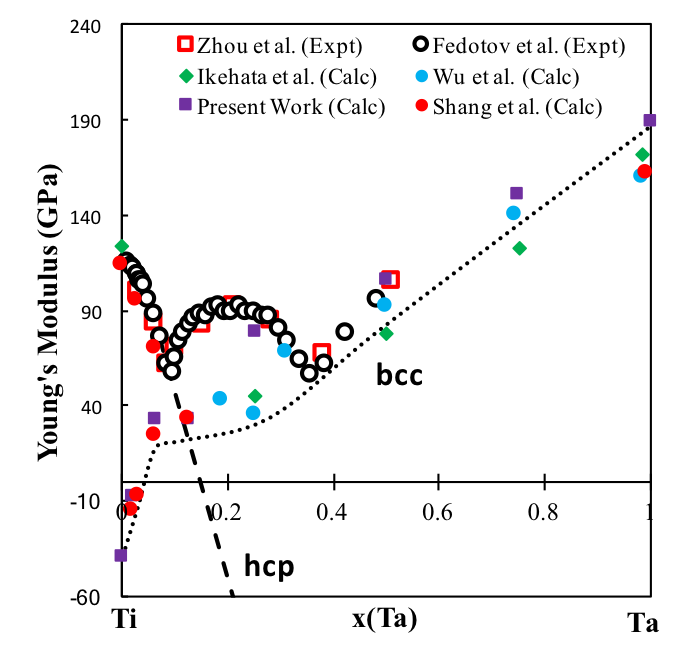
\includegraphics[width=\textwidth]{Chapter-1/Figures/TiTaElastic.png}
	\caption{Comparison of first-principles calculations \cite{Wu2010a,Ikehata2004} and experimental measurements of the Young's modulus of Ti-Ta alloys \cite{Zhou2004a,Zhou2009a,Fedotov1985}. The purple box refers to the composition range when the calculations and experimentally determined $E$ do not match up due to the formation of two metastale phases $\omega$ and $\alpha"$}
	\label{Ch1-figure:titaelastic}
\end{figure}
%%%